\documentclass{article}
\usepackage{amsmath}
\usepackage{graphicx}
\usepackage{hyperref}
\hypersetup{
		colorlinks=true,
		linkcolor=blue,
		filecolor=magenta,
		urlcolor=cyan,
		pdftitle={Overleaf Example},
		pdfpagemode=FullScreen,
	}
\usepackage{float}
\floatstyle{boxed} 
\restylefloat{figure}
\title{Verilog notes}
\date{01-29-2023}
\author{Tommy Bui}

\begin{document}
	\maketitle
	\newpage
	\pagenumbering{arabic}

	\tableofcontents
	\newpage

	\section{Verilog Tutorial}

	\href{https://www.chipverify.com/verilog/verilog-tutorial}{Reference to Chipverify} \newline

	\subsection{Lore}
	In the early days of integrated circuits, engineers had to physically draw transistors \& their netlist on paper. As circuits became more complex and larger in scale, this process eventually tedious. Languages such as VHDL \& Verilog were developed to simply the process of describing the functionality of IC and let tools convert the behavior into hardware using combinational \& sequential logic. \newline

	\subsection{How is Verilog useful}
	Verilog creates a level of abstraction that hides the details of its implementation \& technology. \newline

	E.g. the design of a D flip-flop requires the knowledge of the transistor layout in order to achieve an edge-triggered FF, rise/setup time, fall/clk-Q times to latch value onto flop, etc.

	\section{Introduction to Verilog}
	\href{https://www.chipverify.com/verilog/verilog-introduction}{Source}

	A digital element such as a FF can be represented using combinational gates such as NAND or NOR gates. The functionality of a FF is determined based on the layout of such gates. \underline{How the gates have to be connected is usually determined using K-maps} \newline

	Below is an schemetic of a Data flip-flop \& its corresponding truth table. The output, q is asserted only when rstn \& d are both set. \newline

	\begin{figure}[H]
		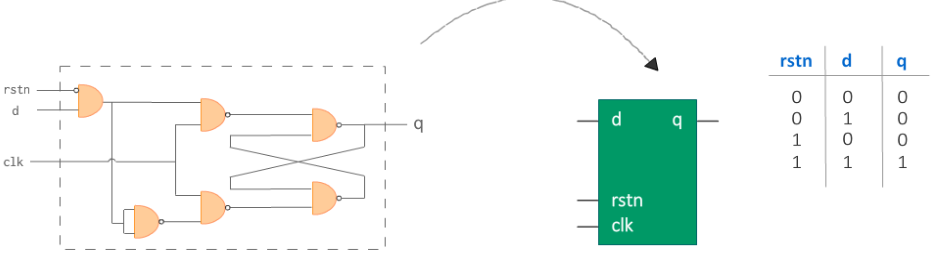
\includegraphics[width=\linewidth]{VerilogPics/figure_1.png}
		\caption{D flip flop}
		\label{D Flip-flop schematic and logic}
	\end{figure}

	\subsection{What is a hardware schematic?}

	A hardware schematic is a daigram that shows how the combinational gates should be connected to implemented a particular behaviour in hardware. From figure 1, a set of NAND gates are connected in order to create a D flip flop. 

	\subsection{What is a Hardware Description Language?}

	It's easier to describe how a block of logic should behave \& let software tools convert that behavior into an actual hardware scchematic. The langugage that describes the hardware functinality is classified as a Hardware Description Language.

	\subsection{Sections of Verilog Code}

	All behavior code should be described within the keywords module \& endmodule. 

	\subsubsection{Verilog section template}
	\begin{itemize}
		\item Module definition \& port list declaration
		\item List of input \& output ports
		\item Declaration of Verilog data types
		\item Module instantiations
		\item Behavioural code
	\end{itemize}

	\begin{figure}[H]
		
\includegraphics[width=\linewidth]{VerilogPics/figure_2.png}
		\caption{Verilog example Template}
		\label{Verilog Template}
	\end{figure}

	\section{Data Types}
	\subsection{Verilog Syntax}

	\href{https://www.chipverify.com/verilog/verilog-syntax}{Source} 
	\href{https://en.wikipedia.org/wiki/Lexical_item}{(Lexical item. In lexicography [citation needed], a lexical item is a single word, a part of a word, or a chain of words ( catena) that forms the basic elements of a language's lexicon (vocabulary)).} \newline \newline

	Lexical conventions in Verilog are similar to C in the sense that it contains a sense of tokens. A lexical token may consist of one or more characters and tokens can be comments, keywords, numbers, strings or white space. However, all lines are terminated by a semi-colon. \newline

	Verilog is case-sensitive, so variables, var\_a \& var\_A differ.


	Two types of comments:
	\begin{itemize}
		\item Single-line comment uses two forward slashes (e.g. //). Single line comments can be nested in a multiple line comment.
		\item Multiple-line comment starts with /* and ends with */ and cannot be nested
	\end{itemize} 
	
	\subsubsection{White space}

	White space refers to spaces, tabs, newlines, \& formfeeds, and is usually ignored by Verilog except when it separates tokens. Be sure to take advantage of this when making readable code. \newline

	\subsubsection{Operators}

	There are three types of operators: unary, binary, \& ternary or conditional. \newline

	\begin{itemize}
		\item Unary operators shall appear to the left of their operand
		\item Binary operators shall appear between their operands
		\item Conditional operators have 2 separate operates that separate 3 operands
	\end{itemize}

	\begin{figure}[H]
		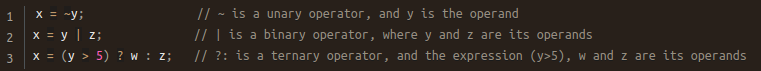
\includegraphics[width=\linewidth]{VerilogPics/figure_3.png}
		\caption{Example of unary, binary, and ternary/conditional operators}
		\label{Example of unary, binary, and ternary/conditional operators}
	\end{figure}

	If the expression (y>5) is true, then variable x will get the value w, else y=z.

	\subsubsection{Number Format}

	\begin{figure}[H]
		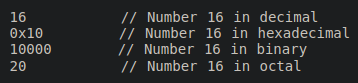
\includegraphics[width=\linewidth]{VerilogPics/figure_4.png}
		\caption{number formats}
		\label{number formats}
	\end{figure}

	By default, Verilog simulators treat numbers as decimals. In order to represent them in different radixes, there are certain rules which must be used. \newline

	\underline{Sized}

	Sized numbers are represented as show below, where size is written only in decimal to specify the number of bits in the number:

	\begin{figure}[H]
		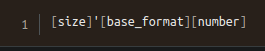
\includegraphics[width=\linewidth]{VerilogPics/figure_5.png}
		\caption{Template for sized numbers}
		\label{Template for sized numbers}
	\end{figure}

	\begin{itemize}
		\item base\_format can be decimal('d or 'D), hex('h or 'H), or octal('o or 'O) \& specifies the base of the number
		\item number can be specified as any valid digit with respect to the specified based format
	\end{itemize}

	\begin{figure}[H]
		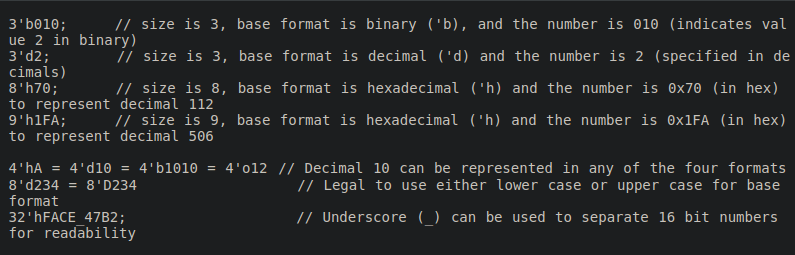
\includegraphics[width=\linewidth]{VerilogPics/figure_6.png}
		\caption{ToDo}
		\label{ToDo}
	\end{figure}

	\underline{Unsized}

	Numbers without a size format specification have a default number of bits depending on the simulator \& machine.

	\underline{Negative} \newline
	Negative numbers are specified with the - sign before the size of a number; It is illegal to have the - between base format \& number.

	\begin{figure}[H]
		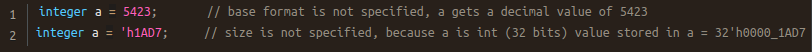
\includegraphics[width=\linewidth]{VerilogPics/figure_7.png}
		\caption{ToDo}
		\label{ToDo}
	\end{figure}
	\underline{Strings} \newline

	A sequence of characters enclosed in double quotes are strings. It cannot be split into multiple lines \& every chracter in the string takes 1B to be stored:

	\begin{figure}[H]
		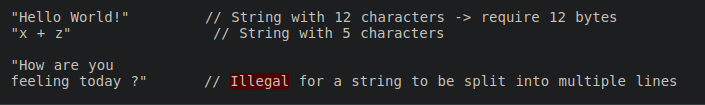
\includegraphics[width=\linewidth]{VerilogPics/figure_8.png}
		\caption{ToDo}
		\label{ToDo}
	\end{figure}
	
	\underline{Identifiers} \newline

	Identifiers are names of variables; Can be made of alphanumeric characters and symbols. They cannot start with a digit nor a \$:

	\begin{figure}[H]
		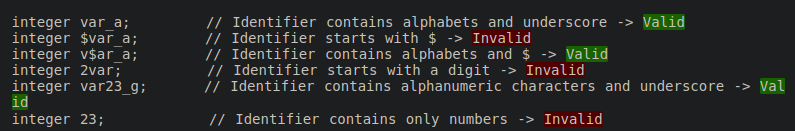
\includegraphics[width=\linewidth]{VerilogPics/figure_9.png}
		\caption{ToDo}
		\label{ToDo}
	\end{figure}

	\underline{Keywords}

	Keywords are special identifiers reserved to be define the language constructs \& are lower case. A list of important keywords is as follows:

	\begin{figure}[H]
		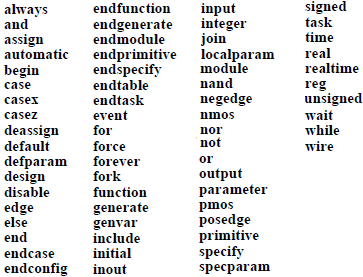
\includegraphics[width=\linewidth]{VerilogPics/figure_10.png}
		\caption{ToDo}
		\label{ToDo}
	\end{figure}

	\underline{Verilog Revisions}
	\begin{figure}[H]
		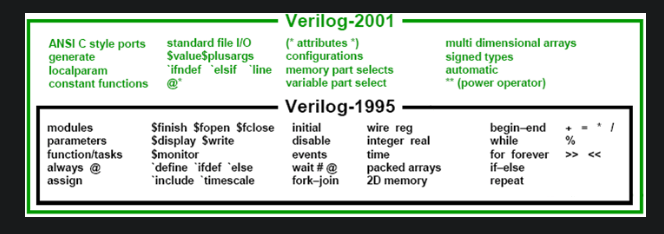
\includegraphics[width=\linewidth]{VerilogPics/figure_11.png}
		\caption{ToDo}
		\label{ToDo}
	\end{figure}

\end{document}
